\chapter{The Finite Volume Method}\label{ch:fvm}
In this section, we present the finite volume method (FVM) for solving nonlinear systems of balance laws, specifically focusing on the shallow water equations (SWE).
Nonlinear problems are more challenging than linear problems, as stability and convergence theory are more difficult to establish.
In particular, when dealing with hyperbolic systems such as the SWE, the presence of discontinuities such as shock waves, hydraulic jumps, and rarefaction waves requires special treatment.
Our focus is on discontinuous solutions, which can accurately capture these shocks and other discontinuities.
The FVM provides a framework for dealing with such solutions in a robust and efficient manner.
Unlike traditional methods, which may struggle to capture sharp gradients or discontinuities, FVM inherently incorporates a mechanism to resolve such features by solving the local Riemann problem at the interfaces between computational cells.
This characteristic makes it particularly well-suited for problems involving abrupt changes in the flow, such as those encountered in the modeling of floods, tsunamis, or dam breaks.

The approach described here is based on the work of LeVeque~\cite{LeVeque2002}, who developed a framework for using the FVM in the context of hyperbolic systems of partial differential equations.
The key idea is to discretize the computational domain into small cells or control volumes and compute the fluxes across the boundaries of these cells.
The solution within each cell is then updated using the information from neighboring cells, ensuring that conservation laws are satisfied.
By solving the local Riemann problem at the cell interfaces, the FVM can accurately capture discontinuities and preserve the sharp transitions between different flow regimes.
In addition to its ability to handle discontinuities, the FVM also has several other advantages, such as its ability to conserve mass, momentum, and energy in a discrete sense.
This property is crucial when solving balance laws, as it ensures that the physical conservation laws are respected even at the discrete level.
The method is also highly flexible, allowing for the use of unstructured grids, which can be beneficial for complex geometries and irregular domains.
Despite its advantages, the FVM also has limitations. The accuracy of the method depends heavily on the choice of numerical flux function and the resolution of the computational grid.
In the presence of strong discontinuities, additional techniques such as limiters or high-order schemes may be required to maintain stability and avoid spurious oscillations.
Furthermore, while the FVM is well-suited for handling hyperbolic problems, it may not be as effective for problems with smooth solutions or for capturing fine-scale features in the solution without sufficient grid resolution.

In this chapter, we derive the finite volume scheme for the 1D SWE and extend it to 2D in cartesian coordinates.
We introduce the MUSCL scheme for higher-order accuracy and discuss the FVM for the 1D linearized SWE in spherical coordinates.
Additionally, we examine the Riemann problem, including the dam break problem, and present numerical flux functions for solving the local Riemann problem at cell interfaces.

\section{The Finite Volume Method for the 1D Shallow Water Equations}\label{sec:FVM_1D_SWE}
We begin by introducing finite volume methods for the SWE in one spatial dimension.
Specifically, we work in the \(x,t\)-plane, discretizing the domain into finite control volumes or cells.
In \autoref{ch:theory}, we derived the integral form for a single control volume \(V = [x_L, x_R] \times [t_1, t_2]\).
Here, we extend this approach to a global domain consisting of multiple cells.
To accommodate this, we update the notation: \(x_{i-1/2}\) and \(x_{i+1/2}\) denote the cell interfaces, while \(t_n\) and \(t_{n+1}\) represent the time levels.
The control volume for cell $i$ at time level $n$ is defined as:
\begin{align*}
    V_i^n = [x_{i-1/2}, x_{i+1/2}] \times [t_n, t_{n+1}],
\end{align*}
where $\Delta x = x_{i+1/2} - x_{i-1/2}$ is the length of the cell and $\Delta t = t_{n+1} - t_n$ is the time step size.
The cell $V_i^n$ is illustrated in Figure~\ref{fig:control_volume_V_i_n}.
\begin{figure}[H]
    \centering
    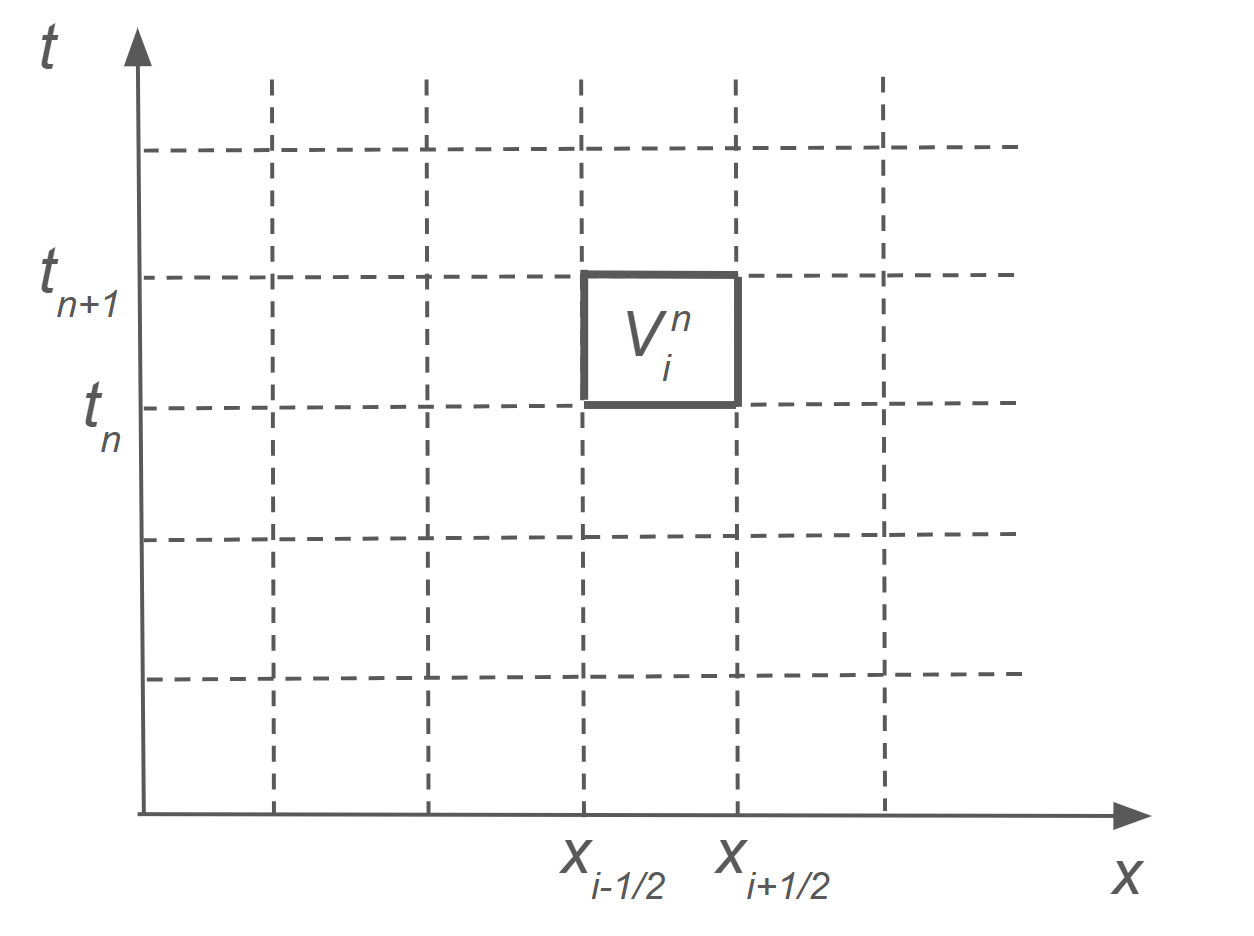
\includegraphics[width=0.4\textwidth]{C:/Users/Matteo/Shallow-Water-Equations/tex/figs/control_volume_V_i_n.png}
    \caption{Illustration of the control volume $V_i^n$ in the $x,t$ plane.}\label{fig:control_volume_V_i_n}
\end{figure}
The grid can be uniform or non-uniform, depending on the application.
For now, we will assume a uniform grid for simplicity.
The finite volume formula is derived from the integral form of the 1D SWE~\eqref{eq:integral_form_1D_final}.
The integral form stated in the new variables ($x_{i-1/2}$, $x_{i+1/2}$, $t_n$, $t_{n+1}$) over the cell $V_i^n$ is given by
\begin{equation}\label{eq:integral_form_1D_SWE_new_variables}
    \begin{aligned}
    \int_{x_{i-1/2}}^{x_{i+1/2}} \mathbf{U}(x,t_{n+1}) \text{ d}x &= 
    \int_{x_{i-1/2}}^{x_{i+1/2}} \mathbf{U}(x,t_n) \text{ d}x + 
    \int_{t_n}^{t_{n+1}} \mathbf{F}(\mathbf{U}(x_{i-1/2}, t)) \text{ d}t -
    \int_{t_n}^{t_{n+1}} \mathbf{F}(\mathbf{U}(x_{i+1/2}, t)) \text{ d}t \\
    &+
    \int_{t_n}^{t_{n+1}} \int_{x_{i-1/2}}^{x_{i+1/2}} \mathbf{S(U)}(x,t) \text{d}x \text{d}t.
    \end{aligned}
\end{equation}
We divide the integral form~\eqref{eq:integral_form_1D_SWE_new_variables} by the cell length $\Delta x$ to obtain
\begin{align*}
    \frac{1}{\Delta x} \int_{x_{i-1/2}}^{x_{i+1/2}} \mathbf{U}(x,t_{n+1}) \text{ d}x &= \frac{1}{\Delta x} \int_{x_{i-1/2}}^{x_{i+1/2}} \mathbf{U}(x,t_n) \text{ d}x\\
    & - \frac{\Delta t}{\Delta x} \left[ \frac{1}{\Delta t} \int_{t_n}^{t_{n+1}} \mathbf{F}(\mathbf{U}(x_{i+1/2}, t)) \text{ d}t
    - \frac{1}{\Delta t} \int_{t_n}^{t_{n+1}} \mathbf{F}(\mathbf{U}(x_{i-1/2}, t)) \text{ d}t \right] \\
    &+ \frac{\Delta t}{\Delta x \Delta t} \int_{x_{i-1/2}}^{x_{i+1/2}} \int_{t_n}^{t_{n+1}} \mathbf{S(U)}(x,t) \text{d}x \text{d}t.
\end{align*}
To simplify the numerical implementation, we introduce cell-averaged values.
These are defined as the averages of the conserved variables $\mathbf{U}$, the fluxes $\mathbf{F}$, and the source terms $\mathbf{S}$ over the volume $V_i^n$.
This leads to the explicit conservative form of the finite volume scheme:
\begin{align}\label{eq:explicit_conservative_1D_SWE}
    \mathbf{U}_i^{n+1} = \mathbf{U}_i^n - \frac{\Delta t}{\Delta x} \left( \mathbf{F}_{i+1/2}^n - \mathbf{F}_{i-1/2}^n \right) + \Delta t \mathbf{S}_i.
\end{align}
%The formula~\eqref{eq:explicit_conservative_1D_SWE} is referred to as a finite volume scheme.
The value $\mathbf{U}_i^n$ is the average value over the $i$-th cell at time $t_n$:
\begin{align*}
    \mathbf{U}_i^n = \frac{1}{\Delta x} \int_{x_{i-1/2}}^{x_{i+1/2}} \mathbf{U}(x,t_n) \text{ d}x,
\end{align*}
also known as the cell average.
The flux $\mathbf{F}_{i-1/2}^n$ is the average flux across the line $x = x_{i-1/2}$ from time $t_n$ to $t_{n+1}$:
\begin{align*}
    \mathbf{F}_{i-1/2}^n = \frac{1}{\Delta t} \int_{t_n}^{t_{n+1}} \mathbf{F}(\mathbf{U}(x_{i-1/2},t)) \text{ d}t,
\end{align*}
and correspondingly the flux $\mathbf{F}_{i+1/2}^n$ is the average flux across the line $x = x_{i+1/2}$ from time $t_n$ to $t_{n+1}$:
\begin{align*}
    \mathbf{F}_{i+1/2}^n = \frac{1}{\Delta t} \int_{t_n}^{t_{n+1}} \mathbf{F}(\mathbf{U}(x_{i+1/2},t)) \text{ d}t.
\end{align*}
The source term $\mathbf{S}_i$ is the average source term over the $i$-th cell at time $t_n$:
\begin{align*}
    \mathbf{S}_i &= \frac{1}{\Delta t \Delta x} \int_{t_n}^{t_{n+1}} \int_{x_{i-1/2}}^{x_{i+1/2}} \mathbf{S}(x,t) \text{ d}x\text{d}t.
\end{align*}
The values are illustrated in Figure~\ref{fig:10_3}.
\begin{figure}[H]
    \centering
    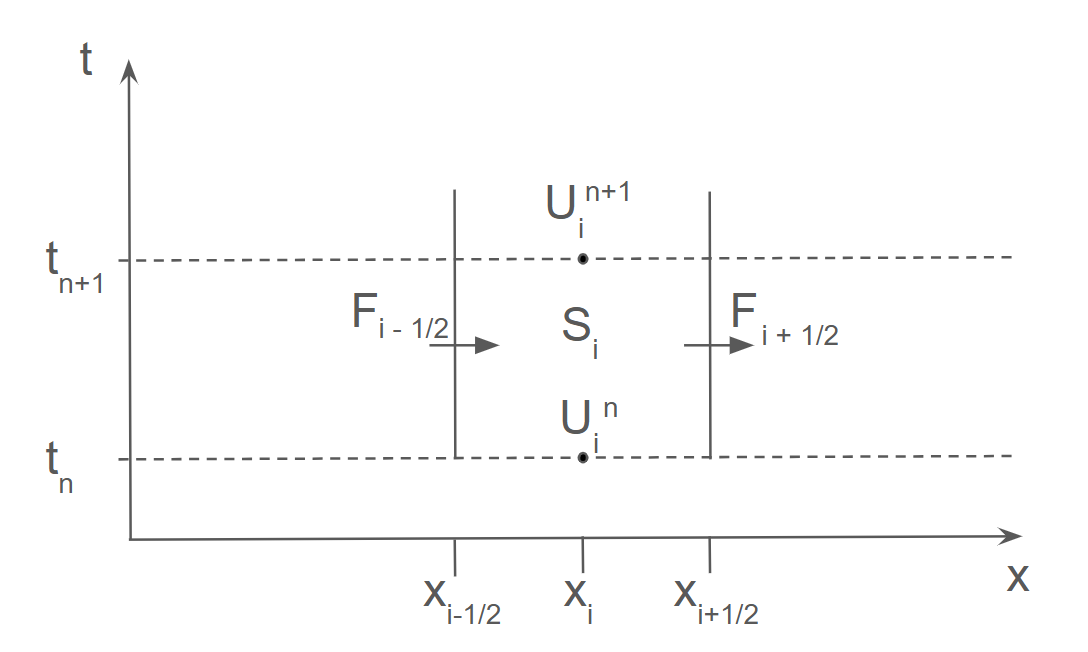
\includegraphics[width=0.5\textwidth]{C:/Users/Matteo/Shallow-Water-Equations/tex/figs/fvm_grid_new.png}
    \caption{Illustration of the grid for the 1D SWE.}\label{fig:10_3}
\end{figure}
The central idea of the FVM is to define the numerical flux $\mathbf{F}_{i+1/2}^n$, at the cell interface, as a function of the cell averages $\mathbf{U}_i^n$ and $\mathbf{U}_{i+1}^n$, since the solution is known only in terms of these cell averages.
Consequently, the FVM does not provide pointwise values of the solution, i.e., $\mathbf{U}(x,t)$, but instead gives cell-averaged values, $\mathbf{U}_i^n$, over the control volume.
One of the main challenges in the FVM is to determine appropiate numerical flux functions that, based on the available cell averages, can reasonably approximate the fluxes at the cell interfaces. 
Later in the thesis, we will consider several numerical flux functions that can be used to solve the local Riemann problem at the cell interfaces.

The finite volume method are closely related to the finite difference method (FDM), but they differs as they are based on the integral form of the conservation laws.
Where finite difference methods tend to break down near discontinuities in the solution, finite volume methods are more suited, since they are based on the integral form of the conservation laws.
The key distinction between the FVM and the FDM lies in their formulation: while the FVM is based on the integral conservation over finite volumes, the FDM is based on satisfying the differential equations point-wise at mesh points.

\section{The Finite Volume Method for the 2D Shallow Water Equations}
We now extend the FVM to two spatial dimensions, meaning we consider both the $x-$ and $y-$direction.
Consider the 2D SWE in vector form~\eqref{eq:vector_form_2D} with $\mathbf{S(U)} = 0$:
\begin{align}\label{eq:2D_SWE}
    \mathbf{U}_t + \mathbf{F(U)}_x + \mathbf{G(U)}_y = 0.
\end{align}
Following the methods outlined in~\cite{Toro2009-Riemann}, an explicit finite volume scheme to solve~\eqref{eq:2D_SWE} is given by
\begin{align}\label{eq:fvm_scheme_2D_unsplit}
    \mathbf{U}_{i,j}^{n+1} = \mathbf{U}_{i,j}^n - \frac{\Delta t}{\Delta x}(\mathbf{F}_{i+1/2,j} - \mathbf{F}_{i-1/2,j}) - \frac{\Delta t}{\Delta y}(\mathbf{G}_{i,j+1/2} - \mathbf{G}_{i,j-1/2}).
\end{align}
This is the unsplit finite volume method, meaning that, in a single step, the cell average $\mathbf{U}_{i,j}^n$ in cell $V_{i,j}$ is updated using the fluxes from all intercell boundaries.
This means, that in each time step, we need to solve the Riemann problem at all cell interfaces, and then use the fluxes to update the cell averages.
The fluxes $\mathbf{F}_{i-1/2,j}$ and $\mathbf{F}_{i+1/2,j}$ are the average fluxes across the lines $x = x_{i-1/2}$ and $x = x_{i+1/2}$.
Correspondingly, the fluxes $\mathbf{G}_{i,j-1/2}$ and $\mathbf{G}_{i,j+1/2}$ are the average fluxes across the lines $y = y_{j-1/2}$ and $y = y_{j+1/2}$.
We work on a domain discretized into rectangular cells of size $\Delta x \times \Delta y$, where $\Delta x = x_{j + 1/2} - x_{j - 1/2} $ and $\Delta y = y_{j + 1/2} - y_{j - 1/2}$.
The fluxes are illustrated in \autoref{fig:FVM_2D_fluxes}.
\begin{figure}[H]
    \centering
    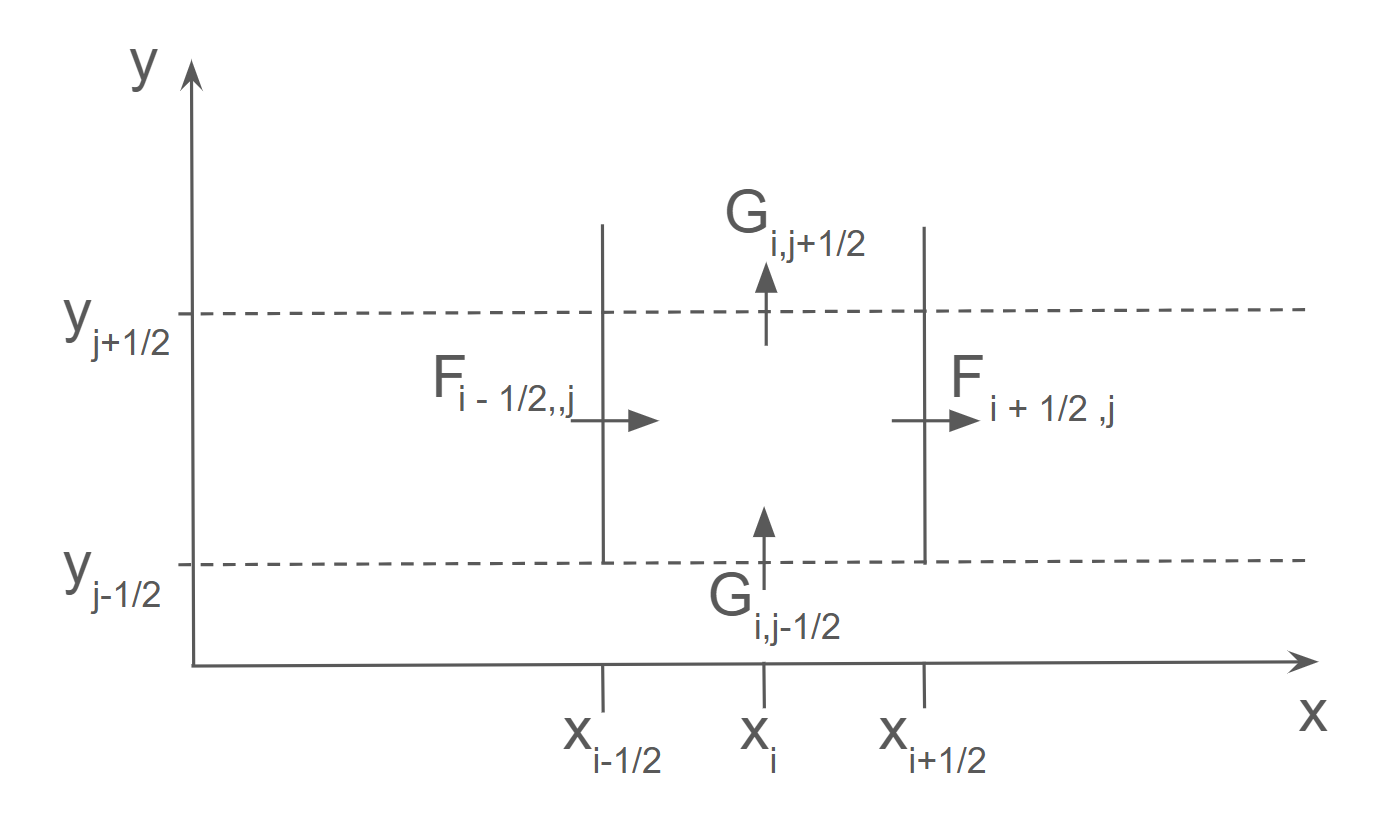
\includegraphics[width=0.5\textwidth]{C:/Users/Matteo/Shallow-Water-Equations/figs/FVM_2D_fluxes.png}
    \caption{Illustration of the fluxes for the 2D SWE.}\label{fig:FVM_2D_fluxes}
\end{figure}
When using the simultaneous update scheme~\eqref{eq:fvm_scheme_2D_unsplit}, we must consider potential stability issues.
%Certain numerical fluxes, such as those from the Lax-Friedrichs, Lax-Wendroff, and FORCE schemes, are not stable in 2D applications.
To address this, several methods can be employed.

The first method we consider is the weighted average flux (WAF) scheme.
The basic WAF scheme, without any nonlinear TVD modification, is prone to oscillations.
To mitigate this, a total variation diminishing (TVD) constraint can be enforced.
To achieve the TVD condition, additional constraints are imposed on the numerical flux or reconstruction process, often through the use of slope limiters.
A limiter function is a technique used to reduce oscillations in the solution, especially near sharp edges or discontinuities, such as shock waves.
For this project, we use the minmod limiter, defined as
\begin{equation*}
    \text{minmod}(a,b) = 
    \begin{cases}
        \max(0, \min(a,b)) & \text{if } a > 0 \\
        \min(0, \max(a,b)) & \text{if } a < 0. 
    \end{cases}
\end{equation*}
Another method we consider is the MUSCL (monotone upwind scheme for conservation laws) scheme.
This method is second-order accurate in both time and space, while the WAF scheme is second-order accurate in space but relies on the time-stepping scheme for temporal accuracy.
The MUSCL scheme, combined with slope limiters, ensures the solution remains satisfies the TVD constraint, effectively preventing oscillations that could occur with high-order spatial discretization near shocks, discontinuities, or sharp changes in the solution.
The key idea in MUSCL is that, instead of using cell averages as in the 1D finite volume method, we reconstruct the solution  in each cell using piecewise first-degree polynomials.
This reconstruction provides a higher-order representation of the solution within each cell.
In this project, we use the MUSCL scheme with the TVD criteria to ensure smooth and stable solutions.
A numerical method $U_{i,j}^{n+1} $ is called TVD if it satisfies the following condition~\cite{LeVeque_1992}:
\begin{align}
    TV(U^{n+1}) \leq TV(U^n),
\end{align}
for all grid functions $U^n$. 
For a discrete function $U_{i,j}$ defined on a grid $i = 0,1, \dots, N$ and $j=0,1, \dots, N$, the total variation $TV(U)$ is defined as
\begin{align}
    TV(U) = \sum_{i=0}^{N-1} \sum_{j=0}^{N-1}  |U_{i+1,j} - U_{i,j}| + |U_{i,j+1} - U_{i,j}|.
\end{align}
The total variation measures the sum of the absolute differences between neighboring grid points.
A TVD scheme ensures that the total variation of the solution does not increase in time, which is crucial for maintaining stability and preventing oscillations.
The TVD property is used in shock-capturing schemes to prevent nonphysical oscillations near discontinuities, helping to accurately capture the shock location.

\section{FVM 1D Linearized SWE spherical}
In this section, we derive the finite volume method for the 1D shallow water equations in spherical coordinates, where we consider the linearized shallow water equations on a circle.
Since we now work on a circle, we must impose periodic boundary conditions.
We follow the same method as in \autoref{sec:FVM_1D_SWE}.
We begin by stating the integral form of the 1D LSWE in spherical coordinates on a global domain.
Each cell has length $\Delta \theta = \theta_{i+1/2} - \theta_{i-1/2}$.
That is, we rewrite~\eqref{eq:integral_form_spherical_1D_final} to be in global variables:
\begin{align}\label{eq:integral_form_spherical_1D_final_global}
    \int_{\theta_{i-1/2}}^{\theta_{i+1/2}} \mathbf{W}(\theta, t_{n+1}) \text{ d}\theta = \int_{\theta_{i-1/2}}^{\theta_{i+1/2}} \mathbf{W}(\theta, t_n) \text{ d}\theta
    - \mathbf{A} \left( \int_{t_n}^{t_{n+1}} \mathbf{W}(\theta_{i+1/2}, t) \text{ d}t - \int_{t_n}^{t_{n+1}} \mathbf{W}(\theta_{i-1/2}, t) \text{ d}t \right).
\end{align}
We divide the integral form~\eqref{eq:integral_form_spherical_1D_final_global} with the cell length $\Delta \theta$ to obtain
\begin{align*}
    \frac{1}{\Delta \theta} \int_{\theta_{i-1/2}}^{\theta_{i+1/2}} \mathbf{W}(\theta, t_{n+1}) \text{ d}\theta &=
    \frac{1}{\Delta \theta} \int_{\theta_{i-1/2}}^{\theta_{i+1/2}} \mathbf{W}(\theta, t_n) \text{ d}\theta \\
    &- \frac{\Delta t}{\Delta \theta} \mathbf{A} \left( \frac{1}{\Delta t} \int_{t_n}^{t_{n+1}} \mathbf{W}(\theta_{i-1/2}, t) \text{ d}t - \frac{1}{\Delta t} \int_{t_n}^{t_{n+1}} \mathbf{W}(\theta_{i+1/2}, t) \text{ d}t\right) .
\end{align*}
Averaging over the terms for a finite volume gives the first-order explicit time-stepping finite volume scheme:
\begin{align}
    \mathbf{W}_i^{n+1} = \mathbf{W}_i^n - \frac{\Delta t}{\Delta \theta} (\mathbf{F}_{i+1/2}^n - \mathbf{F}_{i-1/2}^n).
\end{align}
The scheme uses the cell averages:
\begin{align*}
    \mathbf{W}_i^{n} = \frac{1}{\Delta \theta} \int_{\theta_{i-1/2}}^{\theta_{i+1/2}} \mathbf{W}(\theta, t_n) \text{ d}\theta
\end{align*}
The flux $\mathbf{F}_{i-1/2}^n$ is the average flux across the line $\theta = \theta_{i-1/2}$ from time $t_n$ to $t_{n+1}$:
\begin{align*}
    \mathbf{F}_{i-1/2}^n = \frac{1}{\Delta t} \mathbf{A} \int_{t_n}^{t_{n+1}} (\mathbf{W}(\theta_{i-1/2}, t)) \text{ d}t,
\end{align*}
and correspondingly the flux $\mathbf{F}_{i+1/2}^n$ is the average flux across the line $\theta = \theta_{i+1/2}$ from time $t_n$ to $t_{n+1}$:
\begin{align*}
    \mathbf{F}_{i+1/2}^n = \frac{1}{\Delta t} \mathbf{A} \int_{t_n}^{t_{n+1}} (\mathbf{W}(\theta_{i+1/2}, t)) \text{ d}t.
\end{align*}
%The FVM scheme can be written as 
%\begin{align*}
%    \mathbf{W}_i^{n+1} = \mathbf{W}_i^n - \frac{\Delta t}{\Delta \theta} (\mathbf{A}_{i+1/2}^n - \mathbf{A}_{i-1/2}^n) + \Delta t \mathbf{S}_i,
%\end{align*}
%where $\mathbf{W} = \begin{bmatrix} h \\ u \end{bmatrix}$, $\mathbf{A}_{i+1/2}^n$ is the numerical flux at the cell interface $\theta_{i+1/2}$, and $\mathbf{S} = \begin{bmatrix} 0 \\ fu \end{bmatrix}.$ 
%En eller anden motivation for at bruge denne her metode?? 
The explicit Runge-Kutta 4th order method (ERK4) is a numerical technique used to solve ordinary differential equations (ODEs).
This method is particularly effective for time-stepping and is an alternative approach to traditional time integration schemes.
RK4 provides higher accuracy in time while relying on the same spatial discretization, such as the finite volume method (FVM).
In this context, the RK4 method is applied to numerically solve the linearized 1D shallow water equations in spherical coordinates:
\begin{subequations}
    \begin{align}
        \frac{\partial h'}{\partial t} &= -\frac{h_0}{r \cos\phi} \frac{\partial u}{\partial \theta}, \\
        \frac{\partial u}{\partial t} &= -g \frac{\partial h'}{\partial \theta} - f u,
    \end{align}
\end{subequations}
where \(h'\) is the perturbation in water height, \(u\) is the velocity, \(h_0\) is the mean water depth, \(g\) is the gravitational acceleration, \(f\) is the Coriolis parameter, \(r\) is the Earth's radius, and \(\phi\) is the fixed latitude. 
The ERK4 method employs a four-stage time-stepping scheme to update the solution for $h'$ and $u$.
The general update formula is:
\begin{align*}
    \mathbf{W}_i^{n+1} = \mathbf{W}_i^n + \frac{\Delta t}{\Delta \theta} \frac{1}{6} \left(k_1 + 2 k_2 + 2 k_3 + k_4 \right),
\end{align*}
where the state variable
$\mathbf{W}_i = \begin{bmatrix}
    h_i' \\
    u_i
\end{bmatrix}$ represents the pertubation height and velocity at the $i-$th cell.
The intermediate stages $k_1, k_2, k_3$ and $k_4$ are computed at each time step.
The scheme integrates the equations in time while relying on flux differences to update the solution.
At each time step, the fluxes $\mathbf{F}_i$ between neighboring cells are computed as
\begin{align*}
    \mathbf{F}_i = \frac{1}{2}(\mathbf{F}_{i-1/2} + \mathbf{F}_{i+1/2}),
\end{align*}
where $\mathbf{F}_{i-1/2}$ and $\mathbf{F}_{i+1/2}$ are the fluxes at the edges of the adjacent cells.
These fluxes depend on $h'$ and $u$.
At each ERK4 stage, the fluxes and intermediate derivatives are calculated to ensure accurate time integration.
The final values of $h'$ and $u$ are obtained by combining the contributions from all four stages.
This approach allows the method to achieve high temporal accuracy while maintaining the spatial resolution provided by the finite volume discretization.

%The RK4 scheme approximates the time derivatives of \(h'\) and \(v\) using four intermediate stages:
%\paragraph{Stage 1 (Initial Flux Evaluation):}
%\begin{align}
%    k_{h1} &= -\frac{h_0}{a \cos\phi} \frac{v_\text{flux} - \text{circshift}(v_\text{flux}, 1)}{\Delta \theta}, \\
%    k_{v1} &= -g \frac{h'_\text{flux} - \text{circshift}(h'_\text{flux}, 1)}{\Delta \theta} - f v.
%\end{align}
%Each stage recalculates the fluxes and updates the intermediate derivatives:
%We then update the state variables.The perturbation in water height (\(h'\)) is stored at each time step and visualized as a wave propagating around a great circle on a sphere.

